\documentclass[10pt]{article}
\usepackage[]{ragged2e}
\usepackage{fancyhdr,amsmath,amsthm,amssymb,bbm,graphicx,array,bm,tensor,braket,tikz}
\usepackage[utf8]{inputenc}
\usepackage[letterpaper,left=25mm,right=25mm]{geometry}

\setlength{\parskip}{1em}
\setlength{\parindent}{0em}

\newcommand{\Z}{\mathbb{Z}}
\newcommand{\R}{\mathbb{R}}
\newcommand{\Q}{\mathbb{Q}}
\newcommand{\C}{\mathbb{C}}
\newcommand{\N}{\mathbb{N}}

\DeclareMathOperator{\Ima}{Im}

\linespread{1.25}
\pagestyle{fancy}
\fancyhf{}
\lhead{PHYS 892 $|$  Assignment 1}

\rhead{Dilraj Ghuman $|$ 20191345}

\begin{document}
\textbf{Question 1}

\textbf{1.1} The speed of light is exactly $299792456$ m/s, which rounded to $1\% $ give us $c \approx 3.00\times 10^{8}$. We also know $\hbar \approx 1.05 \times 10 ^{-34} \, \text{m}^{2}\text{kg}/\text{s} = 6.58 \times 10^{-16} \, \text{eV}\cdot \text{s}$ up to $1\% $ error.

\textbf{1.2}

\textbf{(1.2.1)} The given mass is only in units of energy, and we want a dimension of mass. So, we recall that energy is $\frac{[M][L]^{2}}{[T]^{2}}$, where $[M],[L],[T]$ are dimensions of mass, length and time respectively. Then, we see that we only need to get rid of the length/time dimensions twice, which is just our dimensions for $c$, so
\[ 938 \,\text{MeV} \to \frac{938 \, \text{MeV}}{c^{2}} \]
will be the true mass.

\textbf{(1.2.2)} We recall that a unit of energy is the eV, so to get a length from this quantity that has units of energy, we recognize $\hbar$ has units of energy-time and we can get length from the speed of light. That is,
\[ \lambda = \frac{2\pi}{E_{\gamma}} \to \frac{2\pi}{E_{\gamma}}\cdot \frac{\hbar}{c} \]
will be the true wavelength.

\textbf{(1.2.3)} We recall that the dimensions of the inverse square-root gravitational constant are $\frac{[M]^{1/2}[T]}{[L]^{3/2}}$, and we want dimensions of $[M]$. So, we can see that the corresponding factor we need to multiply by to get the units back is $\sqrt{\hbar c}$, since this will have dimensions of $\frac{[M]^{1/2}[L]^{3/2}}{[T]}$ and thus
\[ m_{Pl} = \frac{1}{\sqrt{G}} \to \sqrt{\frac{\hbar c}{G}} \]
as required.

\newpage
\textbf{Question 2}

\textbf{2.1} We first draw what our spherical coordinates will look like relative to the standard euclidean $\{x,y,z\}$ coordinates:
\begin{center}
  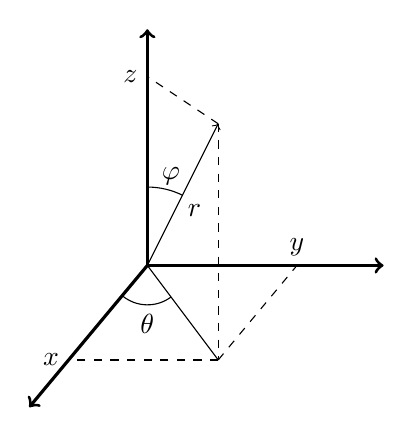
\begin{tikzpicture}
    % Axis xyz
    \draw [->,line width=0.4mm] (0,0) -- (0,3);
    \draw [->,line width=0.4mm] (0,0) -- (3,0);
    \draw [->,line width=0.4mm] (0,0) -- (-1.5,-1.8);
    % vector and r
    \draw [->] (0,0) -- (0.9,1.8);
    \node [below] at (0.6,0.9) {$r$};
    % Projection onto xy
    \draw [dashed] (0.9,1.8) -- (0.9,-1.2);
    % Projection onto z
    \draw [dashed] (0.9,1.8) -- (0,2.4);
    \node [left] at (0,2.4) {$z$};
    % origin to xy projection
    \draw (0,0) -- (0.9,-1.2);
    % projection from xy onto x and y
    \draw [dashed] (0.9,-1.2) -- (-1,-1.2);
    \node [left] at (-1,-1.2) {$x$};
    \draw [dashed] (0.9,-1.2) -- (1.9,0);
    \node [above] at (1.9,0) {$y$};
    % phi arc
    \draw (0.45,0.89) arc [radius=1, start angle=63.4, end angle=90];
    \node [above] at (0.3, 0.9) {$\varphi$};
    % theta arc
    \draw (-0.32,-0.383) arc [radius=0.5, start angle=-130, end angle=-53];
    \node [below] at (0,-0.5) {$\theta$};
  \end{tikzpicture}
\end{center}

which we will convert into the $(r, \theta, \varphi)$ spherical coordinates. Notice we get
\[ x = r\sin(\varphi)\cos(\theta) \quad y = r\sin(\varphi)\sin(\theta) \quad z = r\cos(\varphi) \]
for our conversion. Then, we recall that the metric is $ds^{2} = dx^{2} + dy^{2} + dz^{2}$, so checking each component, we get
\begin{equation*}
  \begin{split}
    dx & = \sin(\varphi)\cos(\theta)dr + r\cos(\varphi)\cos(\theta)d\varphi - r\sin(\varphi)\sin(\theta)d\theta \\
    dy & = \sin(\varphi)\sin(\theta)dr + r\cos(\varphi)\sin(\theta)d\varphi + r\sin(\varphi)\cos(\theta)d\theta \\
    dz & = \cos(\varphi)dr - r\sin(\varphi)d\varphi \\
  \end{split}
\end{equation*}
and we can compute the square to get
\begin{equation*}
  \begin{split}
    dx^{2} & = \sin^{2}(\varphi)\cos^{2}(\theta)dr^{2} + r\sin(\varphi)\cos(\varphi)\cos^{2}(\theta)drd\varphi - r\sin^{2}(\varphi)\cos(\theta)\sin(\theta)drd\theta \\
    & + r\cos(\varphi)\sin(\varphi)\cos^{2}(\theta)drd\varphi + r^{2}\cos^{2}(\varphi)\cos^{2}(\theta)d\varphi^{2} - r^{2}\cos(\varphi)\sin(\varphi)\cos(\theta)\sin(\theta)d\varphi d\theta\\
    & - r\sin^{2}(\varphi)\sin(\theta)\cos(\theta)drd\theta - r^{2}\sin(\varphi)\cos(\varphi)\sin(\theta)\cos(\theta)d\varphi d\theta + r^{2}\sin^{2}(\varphi)\sin^{2}(\theta)d\theta^{2} \\
    dy^{2} & = \sin^{2}(\varphi)\sin^{2}(\theta)dr^{2} + r\sin(\varphi)\cos(\varphi)\sin^{2}(\theta)d\varphi dr + r\sin^{2}(\varphi)\sin(\theta)\cos(\theta)drd\theta \\
    & + r\cos(\varphi)\sin(\varphi)\sin^{2}(\theta)drd\varphi + r^{2}\cos^{2}(\varphi)\sin^{2}(\theta)d\varphi^{2} + r^{2}\cos(\varphi)\sin(\varphi)\sin(\theta)\cos(\theta)d\varphi d\theta\\
    & + r\sin^{2}(\varphi)\cos(\theta)\sin(\theta)drd\theta + r^{2}\sin(\varphi)\cos(\varphi)\cos(\theta)\sin(\theta)d\varphi d\theta + r^{2}\sin^{2}(\varphi)\cos^{2}(\theta)d\theta^{2} \\
    dz^{2} & = \cos^{2}(\varphi)dr^{2} - 2r\sin(\varphi)\cos(\varphi)drd\varphi + r^{2}\sin^{2}(\varphi)d\varphi^{2} \, .\\
  \end{split}
\end{equation*}
So, adding these together and simplifying
\begin{equation*}
  \begin{split}
    ds^{2} & = dx^{2} + dy^{2} + dz^{2} \\
    & = dr^{2} + r^{2}d\varphi^{2} + r^{2}\sin^{2}(\varphi)d\theta^{2} \\
  \end{split}  
\end{equation*}
and the matrix will be
\[
\begin{bmatrix}
  1 & 0 & 0 \\
  0 & r^{2} & 0 \\
  0 & 0 & r^{2}\sin^{2}(\varphi) \\
\end{bmatrix}
\, .
\]

\textbf{2.2} To see this, we recall how the vectors will change under a lorentz transform
\[ A^{\mu} \to \bar{A}^{\mu} = \tensor{\Lambda}{^{\mu}_{\nu}}A^{\nu} \quad A_{\mu} \to \bar{A}_{\mu} = \tensor{g}{_{\mu\nu}}\bar{A}^{\nu} = \tensor{g}{_{\mu\nu}}\tensor{\Lambda}{^{\nu}_{\eta}}A^{\eta} \, .\]

Then, we see that
\[ A^{\mu}B_{\mu} \to \bar{A}^{\mu}\bar{B}_{\mu} = \tensor{\Lambda}{^{\mu}_{\nu}}A^{\nu}g_{\mu\sigma}\tensor{\Lambda}{^{\sigma}_{\eta}}B^{\eta} = \underbrace{\tensor{\Lambda}{^{\mu}_{\nu}}g_{\mu\sigma}\tensor{\Lambda}{^{\sigma}_{\eta}}}_{g_{\nu\eta}}A^{\nu}B^{\eta} = A^{\nu}B_{\nu}\]
and hence we have that the contraction is indeed Lorentz invariant. Moreover, we see
\[ A^{\mu}B_{\mu} = A_{\nu}g^{\nu\mu}B_{\mu} = A_{\nu}B^{\nu} \]
and so the two quantities are the same, as we would expect. 

\textbf{Question 3}

\textbf{3.1} Consider the following table,
\begin{table}[h]
  \centering
  \begin{tabular}{|c|c|c|}
    \hline
     & \textbf{mass MeV} & \textbf{Composition} \\
    \hline
    $p$ & 938.27 & $uud$ \\
    \hline
    $\Lambda$ & 1115.68 & $uds$ \\
    \hline
    $\pi^{-}$ & 139.57 & $d\bar{u}$ \\
    \hline
  \end{tabular}
\end{table}
as required.

\textbf{3.2}

\textbf{3.2.1} In the Lab Frame we will see
\begin{center}
  \begin{tikzpicture}[scale=3]
    % lambda
    \draw [->] (0,0) -- (1,0);
    \draw [->] (0.25,0.25) -- (0.75,0.25);
    \node [left] at (0,0) {$\Lambda$};
    \node [above] at (0.25,0.25) {$P_{\Lambda}$};
    % proton
    \draw [->] (1,0) -- (1.87,0.5);
    \draw [->] (1.3, 0.42) -- (1.7, 0.65);
    \node [right] at (1.87,0.5) {$p$};
    \node [above] at (1.45,0.51) {$P_{p}$};
    % pi-
    \draw [->] (1,0) -- (1.87,-0.5);
    \draw [->] (1.3,-0.42) -- (1.7, -0.65);
    \node [right] at (1.87,-0.5) {$\pi^{-}$};
    \node [below] at (1.45,-0.51) {$P_{\pi^{-}}$};
    % x axis
    \draw [dashed] (1,0) -- (1.5,0);
    % theta
    \draw (1.5,0) arc [radius=0.5, start angle=0, end angle=30];
    \node [right] at (1.5,0.2) {$\theta$};
  \end{tikzpicture}  
\end{center}
but in the COM frame we would see
\begin{center}
  \begin{tikzpicture}[scale=3]
    % lambda
    \node at (0,0) {$\Lambda$};
    % proto
    \draw [->] (0.09,0.05) -- (0.87,0.5);
    \draw [->] (0.34, 0.4) -- (0.775, 0.658);
    \node [right] at (0.87,0.5) {$p$};
    \node  at (0.5,0.7) {$P_{p}$};
    % pi-
    \draw [->] (-0.09,-0.05) -- (-0.87,-0.5);
    \draw [->] (-0.09,-0.34) -- (-0.52, -0.59);
    \node [left] at (-0.87,-0.5) {$\pi^{-}$};
    \node at (-0.2,-0.6) {$P_{\pi^{-}}$};
    % x axis
    \draw [dashed] (0.1,0) -- (0.5,0);
    % theta
    \draw (0.5,0) arc [radius=0.5, start angle=0, end angle=30];
    \node [right] at (0.5,0.2) {$\theta_{p}$};
  \end{tikzpicture}  
\end{center}

\textbf{3.2.2} In the COM frame, we know that $\vec{p}_{p} = \vec{p}$ and $\vec{p}_{\pi^{-}} = -\vec{p}$, and that $\vec{p}_{\Lambda} = \vec{0}$. Using this, we see that

\begin{equation*}
  \begin{split}
    s_{i} & = \left(P_{\Lambda}\right)^{\mu}\left(P_{\Lambda}\right)_{\mu} = E_{\Lambda}^{2} \\
    s_{f} & = \left(P_{p} + P_{\pi^{-}}\right)^{\mu}\left(P_{p} + P_{\pi^{-}}\right)_{\mu} = \left(E_{p} + E_{\pi^{-}}\right)^{2} - (\vec{p} - \vec{p})^{2} = \left(E_{p} + E_{\pi^{-}}\right)^{2} \, .\\
  \end{split}
\end{equation*}

Moreover, we know that
\[ E_{p}^{2} = m_{p}^{2} + p^{2} \quad \& \quad E_{\pi^{-}}^{2} = m_{\pi^{-}}^{2} + p^{2} \]
which gives
\begin{equation*}
  \begin{split}
    E_{p}^{2} - E_{\pi^{-}}^{2} & = m_{p}^{2} - m_{\pi^{-}}^{2} \\
    (E_{p} - E_{\pi^{-}})(E_{p} + E_{\pi^{-}}) & =  m_{p}^{2} - m_{\pi^{-}}^{2} \\
    (E_{p} - m_{\Lambda} + E_{p})m_{\lambda} & = m_{p}^{2} - m_{\pi^{-}}^{2} \\
    E_{p} = \frac{m_{p}^{2} - m_{\pi^{-}}^{2} + m_{\Lambda}^{2}}{2m_{\Lambda}} \\
  \end{split}
\end{equation*}
and in a similar manner we get
\[ E_{\pi^{-}} = \frac{- m_{p}^{2} + m_{\pi^{-}}^{2} + m_{\Lambda}^{2}}{2m_{\Lambda}} \, .\]
The expressions for our momentum come from the relationship used before, that is
\[ p_{p} = \sqrt{E_{p}^{2} - m_{p}^{2}} \quad \& \quad p_{\pi^{-}} = \sqrt{E_{\pi^{-}}^{2} - m_{\pi^{-}}^{2}}\, . \]
Pluggin in some numbers, we get
\[ E_{p} = 943.645 \,\text{MeV} \quad E_{\pi^{-}} = 172.035 \, \text{MeV} \quad p_{p} = 100.58 \,\text{MeV} = p_{\pi^{-}} \, .\]

\textbf{Question 4}

\textbf{4.1}  To show that $\textbf{O}(n)$ is a group under multiplication, we need only show the definition of a group is satisfied. In particular, if $M,N \in \textbf{O}(n)$, notice
\[ MN(MN)^{t} = MN(N^{t}M^{t}) = MNN^{t}M^{t} = MM^{t} = I \implies MN \in \textbf{O}(n) \, ,\]
which is closure (Notice we don't have to show $(MN)^{t}MN = I$ since we showed the inverse of $MN$ is it's transpose and inverses are unique from linear algebra). Next, since $II^{t} = II = I$, we have an identity $I\in \textbf{O}(n)$. Matrix multiplication is associative, and since $\textbf{O}(n) \subset M_{n\times n}(\R)$, we have associativity for free. Finally, we show inverses are also orthogonal. We know they exist, since
\[ \text{det}(MM^{t}) = det(I) \implies (\text{det}(M))^{2} = 1 \implies \text{det}(M) = \pm 1\, .\]
But, since $M$ is orthogonal, by definition $M^{-1} = M^{t}$, so
\[ M^{-1}(M^{-1})^{t} = M^{t}(M^{t})^{t} = M^{t}M = I  \implies M^{-1} \in \textbf{O}(n)\, .\]
So, we can conclude that $\textbf{O}(n)$ is indeed a group.

\textbf{4.2} To show that $\textbf{SO}(n)$ is a group, we need only show that it is a subgroup, so our criterion aren't as restrictive. In particular, we get associativity for free, since $\textbf{SO}(n) \subset \textbf{O}(n)$, and since $\text{det}(I) = 1$, $I \in \textbf{SO}(n)$, and so we have the identity as well. All we need is closure and inverses. Well, notice if $M,N \in \textbf{SO}(n)$, then
\[ \text{det}(MN) = \underbrace{\text{det}(M)}_{1}\underbrace{\text{det}(N)}_{1} = 1 \implies MN \in \textbf{SO}(n) \, .\]
For inverses, we note
\[ \text{det}(M^{-1}) = \text{det}(M^{t}) = \text{det}(M) = 1 \implies M^{-1} \in \textbf{SO}(n)\, .\]
Thus, we have shown $\textbf{SO}(n)$ is indeed a subgroup of $\textbf{O}(n)$.

\textbf{4.3} 

\end{document}
